%# -*- coding: utf-8-unix -*-

\chapter{机票推荐中的冷启动问题}
\label{chap:cold}

冷启动问题一般分为物品冷启动和用户冷启动。前者的含义是当一件物品新添加到物品库中,在还没有用户使用过的情况下如何将其推荐给用户;后者的含义是当一名新用户来到推荐系统,在完全没有用户偏好的情况下如何为用户推荐适当的物品。冷启动问题是推荐系统需要面对的严峻问题。如果处理不好冷启动问题,系统内添加的新物品可能永远都无法向用户推荐;也会影响到新用户的体验,造成用户流失。

在机票推荐系统中,由于机票的数量非常有限并且每条航线上的航班较为固定,通常不会面临物品冷启动问题。而机票本身属于低频、刚需物品。因此机票推荐系统面临的主要问题是用户冷启动问题。在传统的推荐系统中,有一些办法可以解决用户冷启动问题:如在电子商务、书籍网站,用户往往会先提供物品的类别、品牌等信息,随后可以将类别下购买人数的商品推荐给新用户;而在视频、新闻等内容网站,可以在新用户注册时让用户勾选一些感兴趣的主题,即使没有有效获取用户的偏好主题,仍可以将总体最热门的、最实时的内容呈现给用户。

在机票推荐研究领域,由于其业务的特殊性,这两种做法均有不足之处。由于机票具有动态属性,难以静态地描述;并且每个航班的机票数量最多在一两百左右,造成的结果是热门物品与冷门物品之间的差别很小。因此很难单纯以热门程度进行推荐。在第三章,图\ref{fig:res_pref_rec}中的结果表明,以航班热门程度排序的策略难以表现出好的推荐效果。其次,影响用户购买决策的因素有很多,用户每次选购机票时注重的属性可能会因为用户的日程安排、出行目的的不同而发生变动。而在内容网站,用户的兴趣主题一般不会发生频繁变动。

在第三章中,图\ref{fig:user_user_percent}的统计结果表明,在北京-上海这条热门程度很高并且订单、用户数量比最高的航线上,平均每位用户的订单数量仅为两单,仍有$60\%$的用户在过去两年仅订过一单,$90\%$的用户仅订过不多于四单。订单数量在四单及以下的用户占了订单总数的$60\%$。在机票票务服务业务领域,用户冷启动现象也严重影响到用户体验及机票推荐效果。因此需要对冷启动问题展开深入研究。


\section{航线分析及推荐差异}
本小节我们主要对机票推荐中冷启动问题对推荐结果带来的负面影响进行分析与阐述。此处我们仍然选取第三章中提到的四条热门航线进行分析。

\subsection{航线特征分布及用户行为分析}

我们在第三章中提出的机票推荐算法首先将用户数据按照航线进行分割。并为每个用户在每条他选购过机票的航线上独立维护一个偏好模型。这样的做法细化了推荐粒度,使用与目标推荐航线相同的航线来进行建模可以得到更贴合的用户偏好。但是用户的历史订单数据却分散到各个航线。如果在待推荐航线上的训练数据过少,则难以精确刻画用户的偏好。在此我们首先分析航线间的差异;并分析按航线为用户提取偏好对推荐效果带来的影响。

\begin{figure}
\centering
\subfigure[北京-上海航线价格等级分布图]{
 \label{fig:sha-pr}
 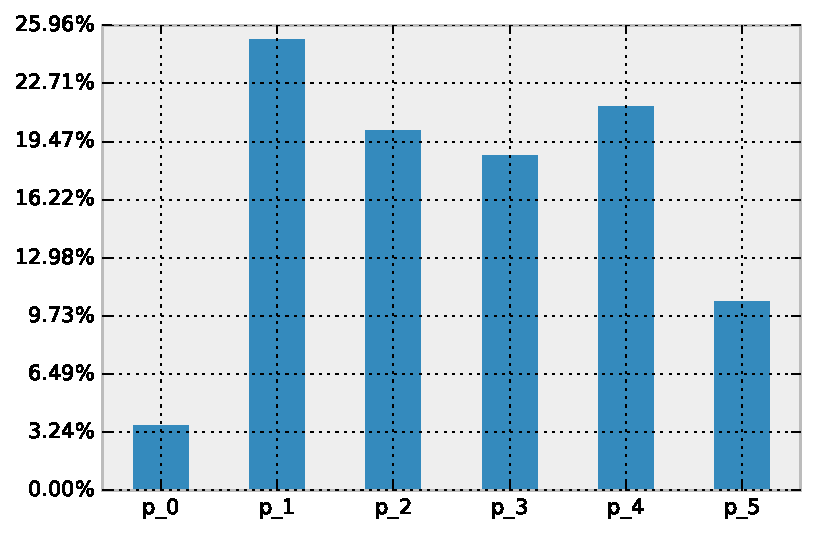
\includegraphics[width=0.49\linewidth]{06/3_pr_dis_bjs.pdf}}
\subfigure[北京-西安航线价格等级分布图]{
 \label{fig:xiy-pr}
 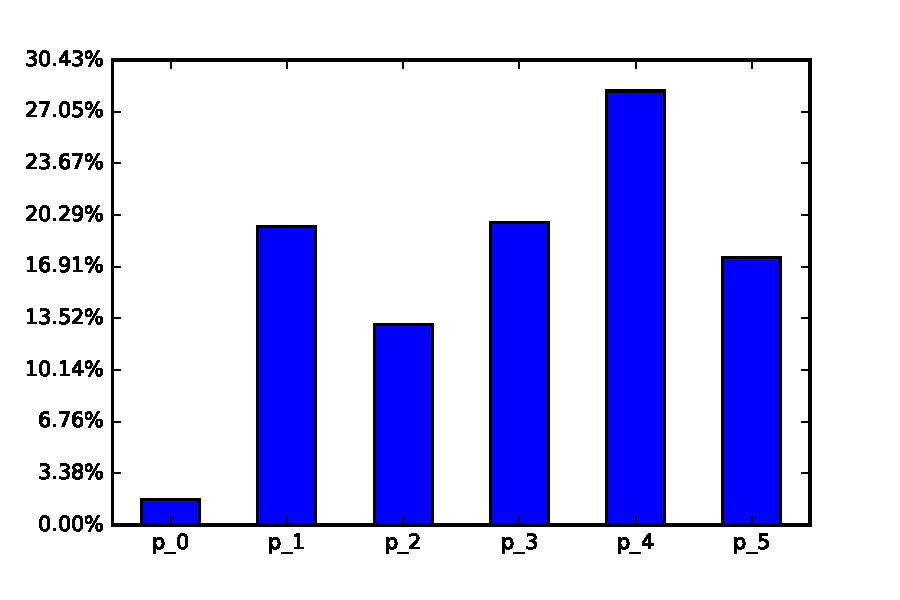
\includegraphics[width=0.49\linewidth]{06/4_pr_dis_xiy.pdf}}
\bicaption[fig:pr_dis]{价格等级分布}{航线间价格指数分布差异}{Fig}{Figure for Variety of  Price Range}
\end{figure}

图\ref{fig:sha-pr}展示了北京到上海航线上的价格指数的分布情况,其横轴的各个标签代表不同的价格指数等级,根据前文提出的价格指数概念,我们将价格指数按照增序划分到$P_0 ~ P_5$六个等级,机票订单价格逐级下降;其纵轴代表位于该价格等级的订单占订单总量的百分比;类似地,图\ref{fig:xiy-pr}展示了北京到西安航线的价格指数分布情况;两图对比可以看出,两条热门航线上价格指数等级的分布占比既有相似之处,也有部分差异。相似之处在于:价格位于最高区间的机票订单数量最少,价格位于最低区间的订单量也较少,而大部分订单集中在中间的价格区间;差异之处在于:在北京到上海航线,高价格区间的订单总体数量占比较大,
其中$P_1$区间的订单总量最多,达到$25\%$;而在北京到西安的航线,低价订单的总体占比较大,
$P_4$区间的订单总量最多。这也与我们之前结合订单、用户数量比得出的航线间出行目的差异相吻合。根据上图的分析我们可以发现,不同航线上的特征分布有所不同。

\begin{figure}
\centering
\subfigure[北京-上海航线航司标准熵分布图]{
 \label{fig:sha-h}
 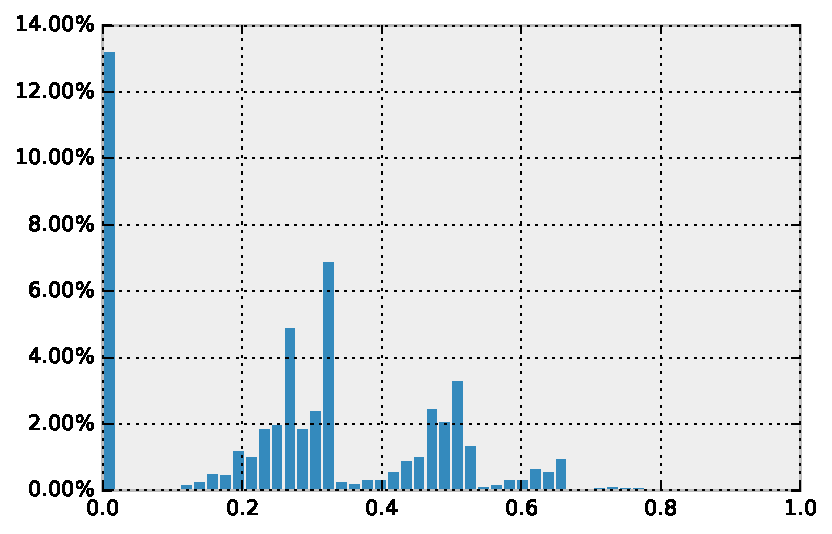
\includegraphics[width=0.49\linewidth]{06/1_entropy_airline_sha.pdf}}
\subfigure[北京-西安航线航司标准熵分布图]{
 \label{fig:xiy-h}
 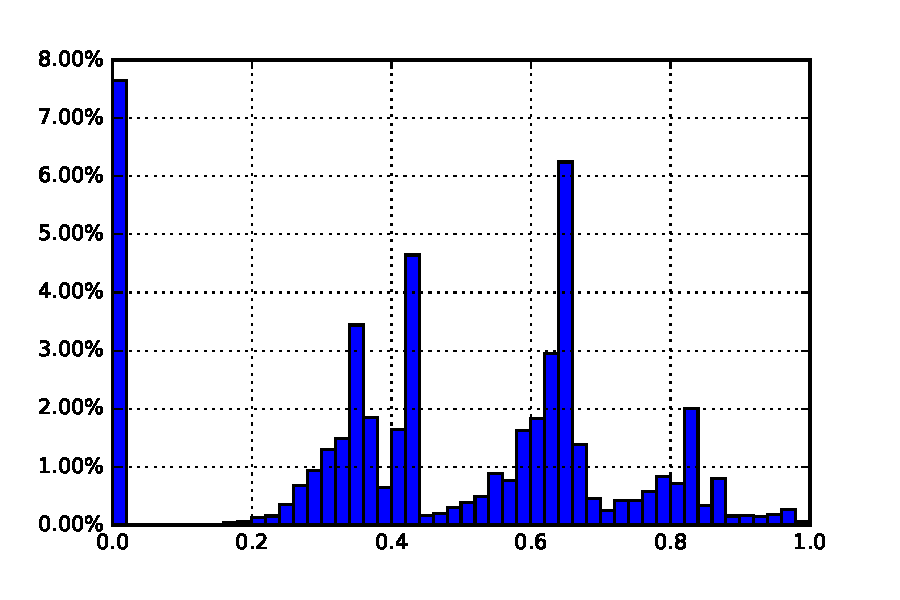
\includegraphics[width=0.49\linewidth]{06/2_entropy_airline_xiy.pdf}}
\bicaption[fig:h_dis]{标准熵分布}{航线间标准熵分布差异}{Fig}{Figure for Entropy Variety of Air Routes}
\end{figure}

图\ref{fig:sha-h}和图\ref{fig:xiy-h}分别展示了北京到上海航线和北京到西安航线的航司标准熵分布图,横轴代表标准熵值,
是将根据公式\ref{eq:entropy}计算出的熵值除以向量的维度进行归一化得到的值。其取值范围在$[0,1]$,用户的偏好集中程度随着熵值的减小而增加。纵轴代表用户的数量占比,即航司偏好的标准熵在该值的用户占用户总数的比例。两条航线都是在标准熵小于0.02的用户数量最多;北京到上海航线上,有更多比例的用户在航司维度的标准熵小于0.02,并且整体熵值偏小,证明在该航线上,用户对航司的偏好更集中。而北京到西安航线,更多的用户集中在0.6附近,相比于前者,用户在该航线上的对航司的偏好更加分散。

至此,我们根据图\ref{fig:pr_dis}反映了不同航线上总体特征分布的差异,这是航线之间客观存在的差异,可能与航空公司的定价策略及票源供给策略等挂钩。还根据图\ref{fig:h_dis}分析了不同航线上用户偏好集中程度的差异,这属于用户主观行为的差异,会受到航线的属性、起飞城市和落地城市的社会性质等因素影响。我们分析对比了客观、主观两个方面的因素对航线造成的影响,也因此造成了航线间的差异。

\subsection{航线差异对机票推荐造成的影响}

分析了航线特征分布及用户偏好集中程度的差异后,需要研究航线间差异对推荐效果的影响。我们的基本思路是使用用户在其他航线的模型为其进行机票推荐,并评估推荐效果。如果使用其他航线模型与仅使用本航线模型的推荐效果相差不多,则证明航线差异不影响机票推荐;反之则证明航线差异对推荐结果的影响不可忽视。

\begin{figure}
 \centering
 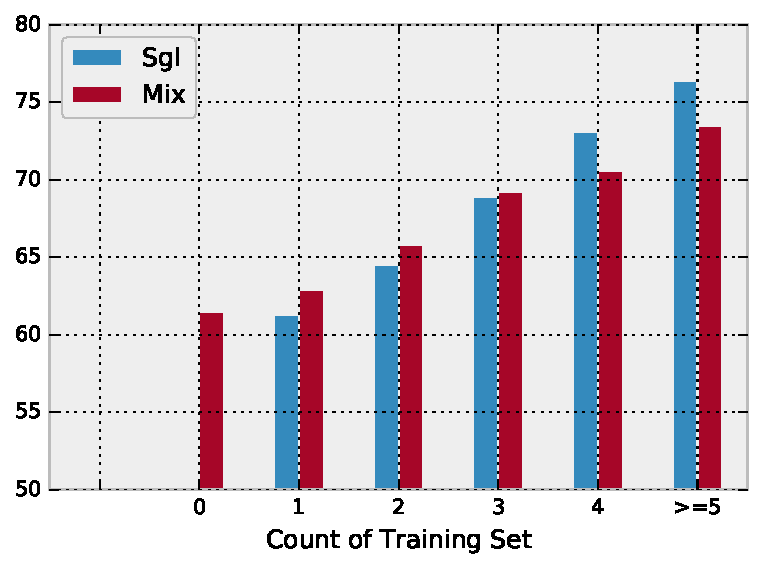
\includegraphics[width=0.75\linewidth]{06/5_res_of_sgl_all.pdf}
 \bicaption[fig:slg_all_rec]{航线推荐效果对比}{单一航线与全航线模型的推荐效果对比}{Fig}{Accuracy of Recommendation for Single and All Air Routes}
\end{figure}

图\ref{fig:slg_all_rec}展示了在北京到上海航线上分别仅使用目标航线历史订单建立用户模型(Sgl,以下称为单一航线模型)以及使用所有航线(包括目标航线)数据建立用户模型(All)进行机票推荐的效果。为了获取有效推荐结果,必须抽取出一条订单作为测试订单,我们将测试订单所在航线定义为目标航线,用户在该航线上其他订单定义为训练订单。对于单一航线模型推荐算法,我们无法为在该航线上只有一条订单的用户进行推荐结果验证。
图的横轴代表用户在目标航线的训练订单条数。纵轴代表推荐平均准确率。对于单一航线模型的推荐算法,其训练订单的数量等于横轴标注的数量;而对于全航线模型推荐算法,训练订单还要再加上用户在其他航线上的历史订单,数目不确定。但在我们要解决的问题中,用户的订单量普遍较为稀少,所以该模型中的总训练订单数量一般不会太大。

从图中我们可以看出,当目标航线训练订单数量为三条及以下时,使用全航线模型的推荐效果好于单一航线模型。两者之间的差距随着订单数量的增加而减小。当目标航线上的训练订单数达到三条时,两种模型的推荐效果没有明显差异,但单一航线模型的计算开销和I/O吞吐开销都较小。当训练订单多于四条时,使用单一航线模型的推荐效果好于全航线模型。由此我们可以得出结论,在用户建模时使用的数据不一定越多越好,由于航线差异可能导致其他航线的用户模型稀释了用户在目标航线上的偏好。为用户按照航线区分特征分布模型对于订单数量在三单以上的用户具有较好的推荐效果。

从图中还可以发现,当目标航线没有训练订单时,全航线模型的机票推荐结果也相当不错,与只有一单训练订单时的单一航线模型推荐结果相差无几。可以说明当用户的订单量较少时,学习的用户模型具有一定的偶然性。并且用户在其他航线上的偏好具备一定程度上的借鉴意义。在实际生产环境中,我们不区分测试订单、训练订单的概念,为了兼顾系统性能与用户体验,可以直接使用该用户在其他航线上的数据进行偏好建模。

\section{航线冷启动问题的分析}
前文我们分析了航线间差异及对个性化机票推荐带来的影响。本节我们针对航线冷启动问题进行研究。航线冷启动问题的含义是用户在需要进行推荐的目标航线上没有历史订单或订单数量较少。根据前文的对照实验结果,我们主要针对的用户是用于建模的目标航线训练订单数量少于三单的用户。

\subsection{航线间差异的量化}

这类用户由于订单量较少,无法在目标航线建立精确的特征分布模型,但在其他航线具有部分订单。为了针对这批用户解决航线冷启动问题,一个基础的思路是我们需要将用户在其他航线上的模型进行适当的修正,使其能够克服航线间的差异,以符合用户在目标航线上的偏好。为此,我们首先需要能够量化航线间的差异程度。

我们仍使用相似度函数来分析航线间的差异。对于结构化的物品。我们可以对其进行特征提取,则物品可以由同构的特征-取值键值对表示。在衡量物品的整体相似度时,可以先按照每个特征的内容组成衡量局部相似度,再将个局部相似度进行融合,就可以得到整体相似度。相似度融合的策略一般是以特征在整体中的相对重要程度定义一个权重指数。因此,整体相似度的衡量公式可以定义为:
\begin{equation}
\label{eq:line_sim}
	Sim(A,B) = \sum_{f \in F}w(f) \times \sigma(f)
\end{equation}

$w_f$代表特征权重。$\sigma_f$是特征局部相似度衡量方法。为机票进行相似度衡量时,机票的每一个特征对应具体数值,我们需要为每个特征所有可能的取值之间定义相似度分数,往往需要借鉴业务领域知识。在航线相似度衡量中,我们可以从与机票类似的角度出发,将航线以多维度特征表示。航线的关键特征与前文提到的特征一致,包括价格、起飞时间、机型、舱位等级、航司和退改签政策。与机票不同的是,航线上的每个特征包含所用用户订单。这里,我们使用航线在每个特征的总体分布向量来代表该航线的对应特征。此外,我们在之前的章节展示了不同航线在用户行为方面有一定的差异,表现在该特征的用户标准熵的分布有较大
差异。因此,用户行为也作为我们衡量航线相似度的一个考虑因素。

航线每个特征的分布可以表示为向量,每个向量所有维度的取值之和为1。我们对特征使用同样的离散化策略。对于航司特征,其种类多达数十种,而每条航线上出现的航司组合不尽相同,往往只有不到十种。如果将所有的航司都罗列到一个向量中,则大多数维度的分布百分比都是0,会对相似度的衡量带来干扰。因此,我们使用字典来维护这个特征。在衡量两条航线在航司的相似度时,我们首先将各自的字典进行扩容,使它们的键包含两条航线上航空公司的并集,可以将航司特征也转化为向量。这里我们使用欧几里德距离作为衡量航线在一个特征上分布差异的公式:
\begin{equation}
	Dist(\mathbf{X},\mathbf{Y}) = \sqrt{\sum_{i=1}^{|X|}(x_i-y_i)^2}
\end{equation}
\begin{equation}
\label{eq:a_sim}
	DistSim(\mathbf{X},\mathbf{Y}) = \frac{1}{Dist(\mathbf{X},\mathbf{Y})}
\end{equation}

欧氏距离衡量了两个向量在空间上的距离,适合在两个相同维度以及量纲的向量之间进行比较。在公式中,$\mathbf{X}, \mathbf{Y}$代表需要计算相似度的向量。式\ref{eq:a_sim}定义了以欧式距离为基础的相似度衡量公式,可以得出当两个向量的欧氏距离为0时,它们的相似度为$1$,且随着欧式距离的增加,向量间相似度递减。
对于用户行为相似度的衡量,结合上一节我们统计过用户熵值分布百分比,我们可以将标准熵在$[0,1]$取值区间内均匀划分为$50$个区间,将每个区间视作一个维度,
将用户熵值在一个特征上的分布也转化为向量,记作$S(f)$。
下公式给出结合航线分布和用户行为的航线间特征相似度衡量方法:
\begin{equation}
	\sigma(f) = DistSim(\mathbf{f_a,f_b}) + DistSim(S(\mathbf{f_a}),S(\mathbf{f_b}))
\end{equation}
\begin{equation}
	\overline{S}(\mathbf{f_a}) = \frac{\ln |f| - S(\mathbf{f_a})}{\ln |f|}
\end{equation}
\begin{equation}
	w(f) = \overline{S}(\mathbf{f_a}) + \overline{S}(\mathbf{f_b})
\end{equation}

$f_a, f_b$是待比较航线上的一个特征,第一项代表航线间特征分布的相似度,第二项代表在该特征上用户行为分布的相似度。每个特征的权重定义为两条航线上该特征分布的标准熵之和。计算出两条航线在所有特征的权重后,将所有值进行归一化就得到了标准权重。至此,我们从特征分布和用户行为两个方面量化了航线间的差异。在解决航线冷启动问题时,可以根据这个量化方法,对用户在非目标航线的模型进行修正,进而将其应用在机票推荐中。

\subsection{最优相似航线的选取及修正模型}
本小节主要介绍我们如何根据航线间差异量化方法为航线冷启动用户选取最优相似航线并进行模型修正。一个最简单的方法是从用户订单中选出与目标航线差异度最小的航线,将用户在该航线的特征分布模型应用在目标航线。这种做法存在几个问题。首先,用户可能在与目标航线相似度最高的航线上也属于冷启动跃用户,这条航线虽然最符合我们的策略,用户在其航线上的特征分布模型也具备相当大的偶然性,因而对提升推荐效果起不到显著作用;其次,虽然选出了与目标航线差异最小的航线,并且用户有足够多的订单,但用户在那条航线上的模型也与该航线的整体特征分布有密切联系,因而无法直接使用在目标航线的推荐中。

鉴于以上几点,我们首先需要选取合适的非目标航线,其次还要对用户在该航线的模型进行修正。为了避免第一个问题,我们在与目标航线相似度的基础上加上用户在本航线的订单数量作为一个激励因子,将航线相似度和订单数量都作为度量因素,提出了加权相似度公式:

\begin{eqnarray}
\label{eq:rsim}
	ReSim(\mathbf{R_a,R_b}) & = & \log{|O_b|} * Sim(\mathbf{R_a,R_b})  \nonumber \\
                        & = & \log{|O_b|} * \sum_{f \in F}w(f) \times \sigma(f)
\end{eqnarray}

式\ref{eq:rsim}在原本相似度公式的基础上添加激励因子,公式中$R_a$代表目标航线,$R_b$代表候选航线,$O_b$代表在候选航线上的订单,我们需要为用户滤掉订单数量不超过一条的航线。在激励因子项我们取订单数量以10为底的对数,避免订单数量对航线相似性的度量造成过大影响。在选取最优航线时,我们将所有非目标航线按照与目标航线的加权相似度进行排序,取出最相似的航线用作模型修正。

用户在目标航线的模型会受到该航线总体特征分布的影响,而特征在不同航线具有不同的总体分布。因此我们在使用非目标航线的用户模型时需要结合航线分布进行修正:
\begin{equation}
\label{eq:adjust-model}
	\mathbf{P'_u} = \sum_{f \in F} \frac{\mathbf{p_f}}{\mathbf{f_a}}
\end{equation}

式\ref{eq:adjust-model}计算了用户的修正特征分布模型。式中,$p_f$代表了用户原本在航线$a$上的模型,$f_a$是航线上该特征的总体分布向量。将用户特征分布除以航线特征分布就可以得到与航线分布无关的用户模型。例如,用户在某特征的分布占比分别为$[20\%,30\%,30\%,20\%]$,在本航线上该特征总体分布是$[10\%,40\%,20\%,30\%]$,则修正后的用户特征分布占比为$[2,0.75,1.5,0.67]$,最后对修正模型进行归一化。

得到用户在最优相似航线的修正模型后,我们将修正模型与用户在目标航线上的模型进行整合。若用户在目标航线没有历史订单,则可以直接使用修正模型;否则,由于用户在目标航线建模使用的订单数量很少,而学习修正模型使用的订单较为充足,并且修正模型也去除了不同航线分布产生的影响,最大限度地降低了模型差异。我们可以将两个模型按等权重线性相加,得到结合最优相似航线的修正混合模型,就可以使用该模型为用户做机票推荐。

\begin{algorithm}
\caption{航线冷启动用户修正混合模型}
\label{algo:air_cold_dis}
\begin{algorithmic}[1]
\Require
\Statex 用户全航线历史订单 $O$
\Statex 机票特征集合 $F$
\Statex 目标推荐航线 $r_a$
\Statex 各航线总体特征分布 $M$

\Ensure 
\Statex 修正混合特征分布模型 $D_{mix}$

\State $P \gets routePartition(O,r_a)$;
\For { $r \in P$}
\State $D[r] \gets extractDistribution(O_r,F)$;
\State $W[r] \gets getWeight(O_r,F)$;
\EndFor

\State $r_o \gets getOptimalRoute(P)$
\State $D'[r_o] \gets D[r_o] / M[r_o]$

\State $D_{mix} = Normalize(D[r_a] + D'[r_o])$

\State \Return $D_{mix}$
\end{algorithmic}
\end{algorithm}

算法\ref{algo:air_cold_dis}展示了航线冷启动用户获取修正混合模型的过程。在第三章中,算法\ref{algo:pref_cal}的输入数据用户在目标航线数据,而本算法的输入数据是用户全航线数据,还需要航线总体特征分布数据。将历史订单按航线进行划分后分别计算特征分布模型以及对应特征权重。再根据式\ref{eq:rsim}计算航线间相似度,将相似度最高的非目标航线进行模型修正,最后与用户在目标航线上的模型进行相加及归一化即得到修正混合模型。后续推荐流程与第三章总算法描述相同,本节不再赘述。

\subsection{实验结果分析}

\subsubsection{实验数据集及评价指标描述}

本节我们根据数据实验来测试为航线冷启动用户应用修正混合模型的推荐准确率。
我们仍选取北京到上海,北京到成都,北京到深圳,北京到西安这四条航线。为了符合航线冷启动场景,我们选取了在目标航线上训练订单数量不超过两单并且具有在其他航线的历史订单数量不少于三单的用户。我们为这些用户分别测试单一航线用户模型、全航线用户模型以及修正混合模型的推荐效果。

实验评价指标与第三章中相同,我们使用式\ref{eq:a-rec}对每条机票推荐准确率进行评价,
使用式\ref{eq:ma}对为所有用户使用三种模型的推荐的平均准确率进行评价。

在图\ref{fig:slg_all_rec}中我们可以看出,即使用户在目标航线仅有一旦训练订单,推荐效果也远好于第三章实验章节中提到的低价排序和热度排序策略。因此,对于这两种以基本业务策略进行机票推荐的模型,这里不再测试其效果。

\subsubsection{航线间相似度分析}

\begin{table}[!hpb]
  \centering
  \bicaption[tab:airline_sim]{相似度结果}{四条航线之间的相似度结果}{Table}{Similarity Between Test Air Routes}
  \begin{tabular}{|c|c|c|} \hline 
    航线1& 航线2 & 相似度\\ \hline
    BJS-SHA & BJS-CTU & 55.4\% \\ \hline
    BJS-SHA & BJS-SZX & 50.5\% \\ \hline
    BJS-SHA & BJS-XIY & 47.6\% \\ \hline
    BJS-CTU & BJS-SZX & 61.8\% \\ \hline
    BJS-CTU & BJS-XIY & 49.0\% \\ \hline
    BJS-SZX & BJS-XIY & 49.6\% \\ \hline
  \end{tabular}
\end{table}

表\ref{tab:airline_sim}分析使用式\ref{eq:line_sim}对航线相似度的衡量情况。相似度数值已经就参与衡量的特征数量做了归一化。从个表格中可以得出,北京到成都和北京到深圳具有最高航线相似度,为$61.8\%$;而北京到上海和北京到深圳之间的航线相似度最低。在四条航线中,北京-成都与其他三条航线的相似度都很高,而北京-西安与其他航线的相似度都较低。另外,此处相似度没有考虑航线订单数量激励因子,是航线间总体特征分布和用户标准熵分布相似度的融合。当为航线冷启动用户挑选最优航线时,如果用户在与目标航线相似度非最高航线上的订单数量超过相似度最高的航线,根据带激励因子的航线相似度公式,前者可能会排在更靠前的位置。因此对不同的用户会产出不同的排序结果。前文提到,在订单数量较少的情况下,学习到的用户特征分布模型可能会具有偶然性。

\subsubsection{用户模型与航线特征分布相关性分析}

在偏好模型修正章节,我们为了使用户在不同航线上的特征分布模型摆脱航线总体特征分布的影响,提出了对用户模型根据该航线的特征分布进行修正的方法,本小节我们将对用户模型与航线特征分布的相关性进行分析。我们使用皮尔逊系数来计算向量间的相关性:

\begin{eqnarray}
	r(X,Y)  & = & \frac{\sum(X-(\overline{X}))(Y-(\overline{Y}))}{(\sqrt{\sum(X_i-(\overline{X}))^2}\sqrt{\sum(Y_i-(\overline{Y}))^2})} \nonumber \\
	& = & \frac{n\sum(X_iY_i)-\sum X *\sum Y}{\sqrt{n\sum X_i^2 - (\sum X_i)^2}\sqrt{n\sum Y_i^2 - (\sum Y_i)^2}}
\end{eqnarray}

X,Y是两个等维度的向量,皮尔逊系数的取值在$[-1,1]$之间。当X,Y呈正相关时,X与Y的增减性相同,此时,皮尔逊系数的取值在$(0,1]$;
当X,Y呈负相关时,X与Y的增减性相反,皮尔逊系数的取值范围在$[-1,0)$。X,Y的相关性越强,相关系数的绝对值越接近1。

\begin{figure}
 \centering
 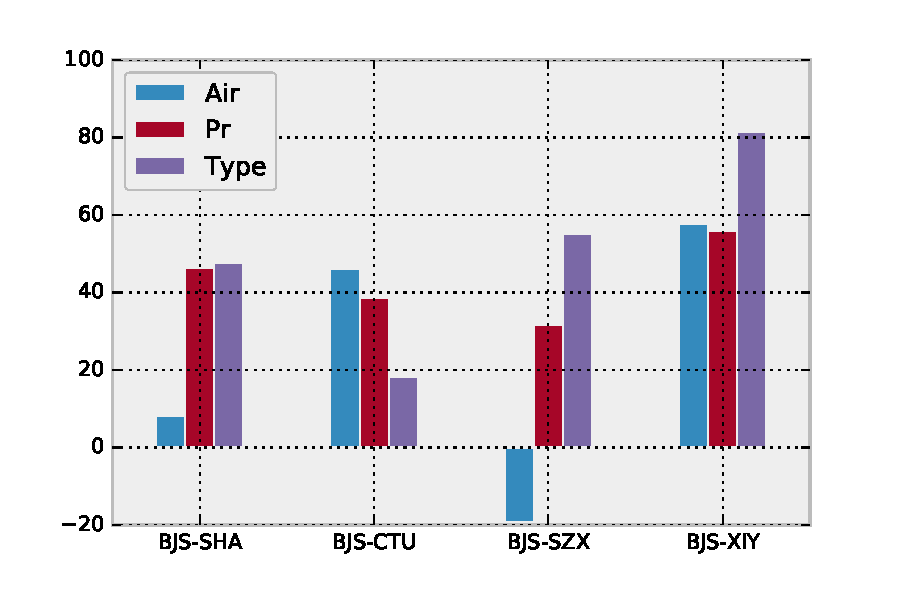
\includegraphics[width=0.75\linewidth]{06/7_res_of_pear_.pdf}
 \bicaption[fig:pear_cof]{相关系数}{用户模型与航线分布相关系数}{Fig}{Pearson Correlation Coefficient between User Model and Distribution over Air Routes}
\end{figure}

图\ref{fig:pear_cof}展示了航空公司、价格等级、飞机型号三个特征与四条航线上特征分布的相关程度。其中纵轴的含义是相关系数百分比。此处使用了北京到西安航线上的用户偏好模型,我们在该航线上对活跃用户(训练订单不少于三单)进行抽样;并计算他们的特征分布模型在这三个维度上与四条航线的相关系数的平均值。从图中可以看出,用户在北京到西安航线上的模型与该航线的特征分布相关程度最高,均远高于其他航线。在三个特征中,相关程度差异最小的是价格等级特征,因为无论在哪条航线上,经济舱、低价机票用户的比例都是最高的;相关程度差异最大的是航空公司特征,这可能与不同航空公司在不同航线的运营策越有关。
在北京-深圳航线,用户模型与航线特征分布呈负相关。我们通过计算相关系数验证了用户模型与航线特征分布的关系。

\subsubsection{航线冷启动用户机票推荐结果分析}

\begin{figure}
 \centering
 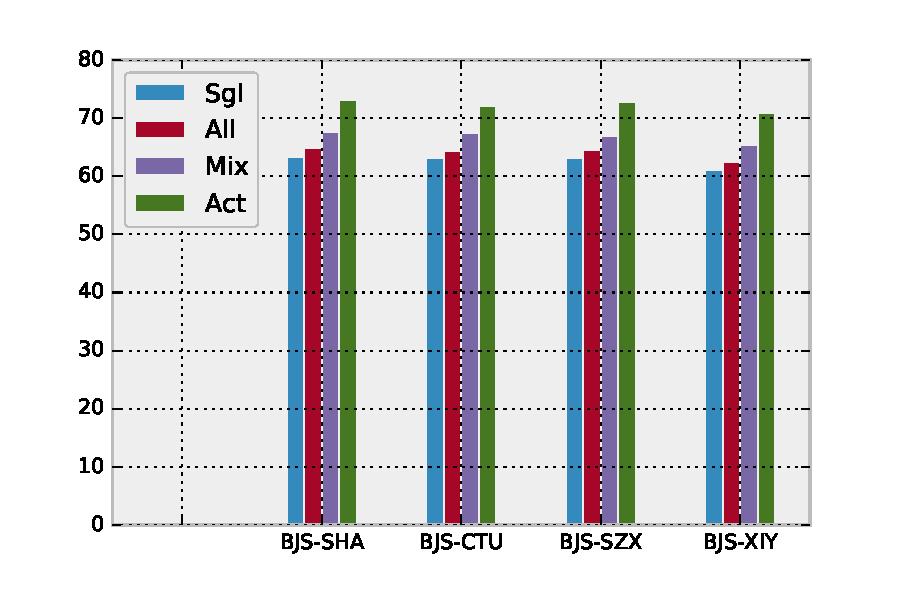
\includegraphics[width=0.75\linewidth]{06/6_res_of_air_cold_rec.pdf}
 \bicaption[fig:cold_rec]{航线冷启动推荐}{航线冷启动用户推荐结果}{Fig}{Mean Accuracy of Recommendation for Air Route Cold Start Users}
\end{figure}

图\ref{fig:cold_rec}展示了在四条航线上的机票推荐结果。其中Act标签代表为该航线活跃用户的单一航线模型推荐结果。可以看到,在每条航线上,活跃用户的机票推荐准确率比非活跃用户提升较多。Sgl标签代表为航线冷启动用户使用单一航线模型的推荐结果;All标签代表为航线冷启动用户使用全航线模型的推荐结果;Mix代表为航线冷启动用户使用修正混合模型的推荐结果。我们得出基本结论是为此类用户使用全航线模型的推荐准确率高于仅使用目标航线模型;而使用修正混合模型具有最高的推荐准确率,只是距活跃用户仍有一定差距。


\section{基于社会关系解决用户冷启动问题}

本节我们分析用户冷启动问题,即该用户的活跃程度较低,在所有航线上的订单数量都很少。因此我们无法使用上一节中选取最优相似航线的方法为用户建立修正混合模型。唯一可行的方法似乎只有使用用户全航线模型进行推荐,但这样同样面临上一节中提到的航线间特征分布差异、用户行为差异的问题。为了有效解决这类问题,我们借助于用户间的社会关系,通过模型迁移来强化非活跃用户的特征分布模型。


\subsection{社会关系的定义}
在现实生活中,社会关系用于描述人与人之间的社会联系,例如家庭、同事、朋友等。在机票推荐情景中,我们无法获得用户之间的在现实中的具体关系,也难以衡量用户之间社会关系的亲疏程度。然而,我们可以通过机票订单数据集挖掘到用户之间的关系,这种关系仅表示用户在机票票务领域的一种连接形态,虽不能反映用户间的现实社会关系,但在解决用户冷启动问题中可以提供一定程度的帮助。

在机票的订购流程中,当用户选定机票后,需要填写乘客的身份信息,包括姓名、证件号等内容,因此进行订票的网站用户不一定是最终的乘客。用户与乘客之间可以是一对一、一对多、多对多这几种类关系;在数据集中,我们通过网站账户的注册ID来识别用户;通过加密过的乘客证件号来识别乘客。如果一个乘客出现在多个用户中,我们称这两个用户具有共同乘客,可以为这两个用户建立社会关系。在共同乘客数量的统计过程中,我们可以使用倒排索引以大幅减少计算开销。在全量订单中统计乘客-用户字典,以乘客为键,乘客出现过的用户集合为值,为集合中的用户两两增加一次共同乘客数量。对所有乘客都执行统计后,
我们就可以得到所有用户的共同乘客数量。

挖掘用户间的社会关系除了依据用户与乘客的对应关系外,乘客之间还有同乘关系。虽然他们没有在同一个用户下订票,却乘坐了同架飞机。如果两个用户同乘飞机超过一次,我们就可以认为两个用户可以建立社会关系。这里我们按同航班号、同起飞日期、同舱位等级的策略来标识同架飞机。因为两个同乘的用户一般不会选择不同的舱位,这里可以大幅减少我们的计算开销;并且我们的目的是根据用户间的社会关系强化用户模型,如果同乘用户的偏好具有较大差异,他们的模型也不应该被相互迁移。

\begin{figure}
 \centering
 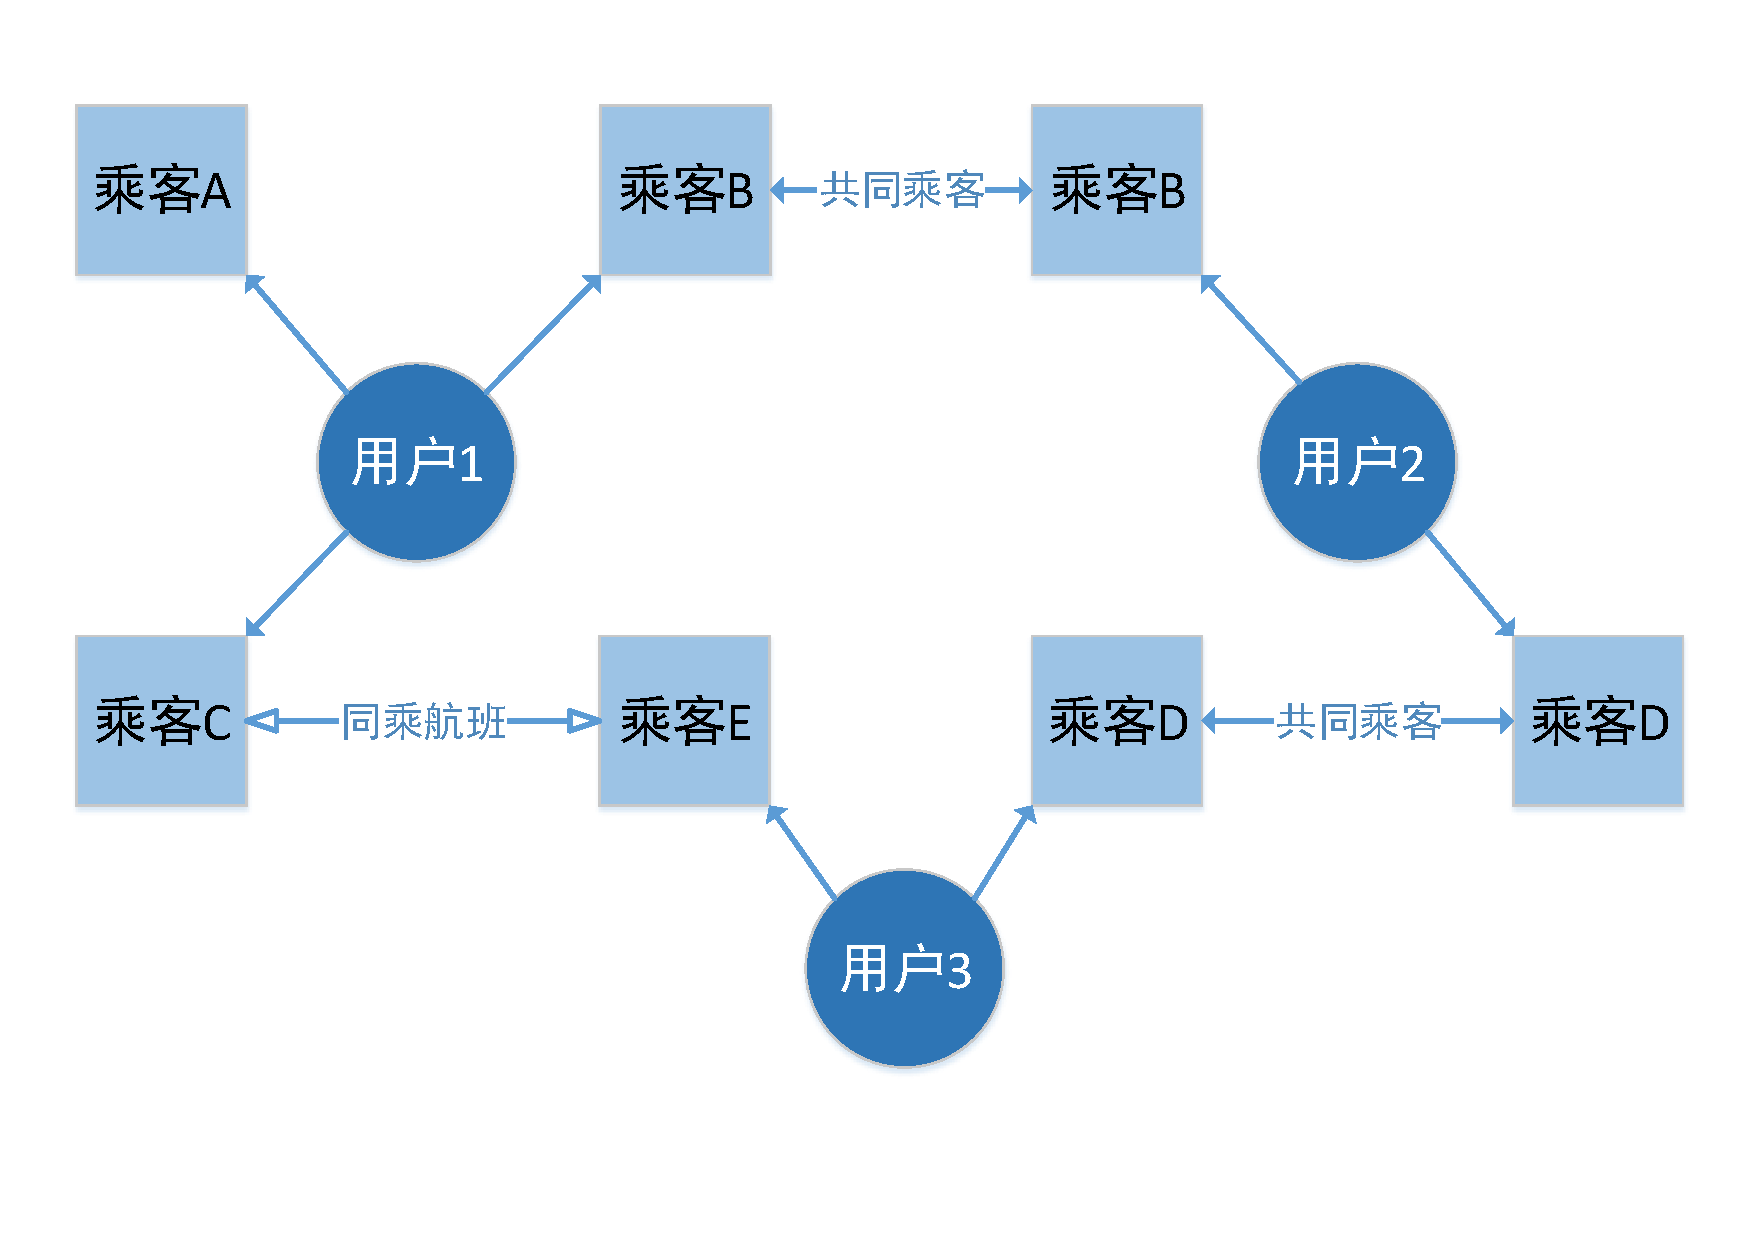
\includegraphics[width=0.75\linewidth]{06/8_model_of_social.pdf}
 \bicaption[fig:social_model]{用户社会关系}{用户间社会关系模型}{Fig}{Model of Social Relationship among Users}
\end{figure}

图\ref{fig:social_model}阐述了从机票订单中挖掘出的用户社会关系模型。图中共有三位用户以及五位乘客。其中用户一为乘客A、B、C订过机票;用户二为乘客B、D订过机票;用户三为乘客D、E订过机票。因此用户一和用户二可以通过乘客B建立社会关系;用户二和用户三通过乘客D建立社会关系。乘客C和乘客E曾同乘飞机超过一次,也可在用户一和用户三之间建立社会关系。

在定义了机票用户之间的社会关系后,我们还需定义计算社会关系紧密程度的衡量规范。当某个冷用户可以与多个用户建立社会关系时,我们可以按照这个衡量规范为其挑选关系最紧密的用户进行模型增强。例如在上图\ref{fig:social_model}中,虽然用户一和用户三都与用户二有共同乘客,但是用户三包含的乘客数少于用户一,我们可以认为用户三与用户二的社会关系紧密度高于用户一和用户二。在选择强化用户二的偏好模型时,用户三有更高的优先级。

\begin{equation}
\label{eq:relation}
	Rela(U_1,U_2) = \log|O_{U2}| \frac{UF(U_1,U_2) + UP(U_1,U_2)}{\sqrt{|P_{U1}|*|P_{U2}|}}
\end{equation}

式\ref{eq:relation}从共同乘客数量和同乘次数两方面衡量了用户间的社会关系紧密度。分子中$UF(U_1,U_2)$代表两个用户的同乘(User-Flight)次数;
$UP(U_1,U_2)$代表两个用户共同乘客(User-Passenger)数量。分母是用户包含的乘客数量乘积,
是一项惩罚项,其含义是当UF,UP数量固定时,一个用户包含的乘客数量越大,这个用户的偏好越不具备代表意义,因此使用这个偏好为冷启动用户进行模型增强的意义很低,我们需要将这类用户与其他用户的关系紧密度定义的尽量小。如果组成两个账户的乘客完全相同,则他们的关系紧密度不小于1;在分子$UF(U_1,U_2)$中,我们不存储同乘次数仅为1次的用户,因为每架飞机都有数百位乘客共同出行过,我们不能认为这些乘客之间都互相具备社会关系。

我们假设U1代表冷启动用户,称为源用户;U2代表需要为U1进行模型增强的候选用户。公式中第一项是候选用户的订单数量取以10为底的对数。正如同我们在解决航向冷启动问题时添加的激励因子,需要保证候选用户不是冷启动用户。

\subsection{增强用户模型}

定义了用户间社会关系以及社会关系紧密度计算公式后,我们就可以针对具有社会关系的冷启动用户进行模型增强。将与该用户建立社会关系的用户集合以社会关系紧密度由高到低进行排序。取排序最靠前的用户为目标用户进行模型增强。

如果候选用户在目标航线上不是冷启动用户,则将候选用户的特征分布模型与源用户的模型线性相加;反正,则采取类似航线冷启动用户的模型修正策略,将候选用户在与目标航线最相似航线上的模型与源用户的模型相加。

\begin{algorithm}
\caption{增强用户模型}
\label{algo:all_cold}
\begin{algorithmic}[1]
\Require
\Statex 用户全航线历史订单 $O$
\Statex 机票特征集合 $F$

\Ensure 
\Statex 增强用户特征分布模型 $D_{amp}$

\State $U \gets getRelatedUsers(u_a)$
\State $Rank\_list \gets \emptyset$
\For { $u \in U$}
\State $Rank\_list.append(Rela(u_a,u)) $
\EndFor
\State $u_o \gets Max(Rank\_list)$
\State $r_o \gets getOptimalRoute(u_o)$
\State $D'[r_o] \gets D[r_o] / M[r_o]$

\State $D_{amp} = Normalize(D[r_a] + D'[r_o])$

\State \Return $D_{amp}$
\end{algorithmic}
\end{algorithm}

算法\ref{algo:all_cold}描述了冷启动用户模型增强的过程。第一步需要获取与该用户建立社会关系的用户集合。然后根据关系紧密度公式挑选出与源用户社会关系最紧密的候选用户。最后将候选用户在目标航线或最优相似航线上的特征分布模型对用户模型进行增强,并将增强后的模型用于机票推荐。

\subsection{实验结果分析}

\subsubsection{实验数据集及评价指标描述}

本节我们验证增强用户模型为冷启动用户进行机票推荐的准确率。仍旧选取北京到上海,北京到成都,北京到深圳,北京到西安这四条航线。选取了在每条航线上订单数量均不超过两单的用户,这些用户还要具备可建立社会关系的其他候选用户。我们为这些用户分别测试单一航线用户模型、全航线用户模型以及增强用户模型的推荐效果。

我们仍旧使用式\ref{eq:a-rec}对每条机票推荐准确率进行评价,
以及式\ref{eq:ma}对每种模型下所有用户的推荐平均准确率进行评价。

\subsubsection{用户社会关系分析}

\begin{figure}
 \centering
 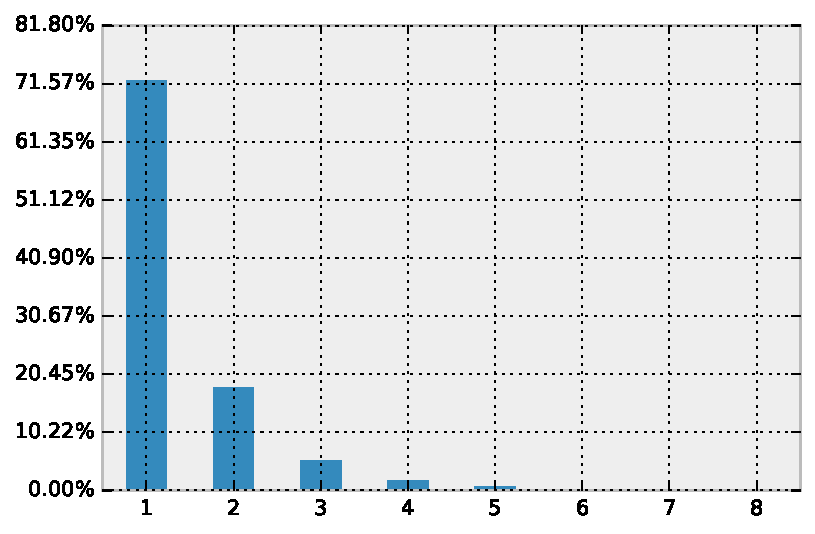
\includegraphics[width=0.75\linewidth]{06/9_same_flight.pdf}
 \bicaption[fig:same_flight]{同乘用户}{具备同乘关系的用户分布图}{Fig}{Users Establishing Relationship with Others for taking Same Flight}
\end{figure}

图\ref{fig:same_flight}描述了通过同乘航班建立社会关系的用户分布图。其横轴代表与一个用户有同乘关系的用户数量。前文提到,具备同乘关系的前提是与其他用户乘坐同一航班超过一次。可以看到,只与一位用户有同乘关系的用户数量占比达到70\%,与两位用户有同乘关系的用户数量占比约18\%左右,与三位以上用户有同乘关系的用户数量占比约10\%。

\subsubsection{冷启动用户机票推荐结果分析}

\begin{figure}
 \centering
 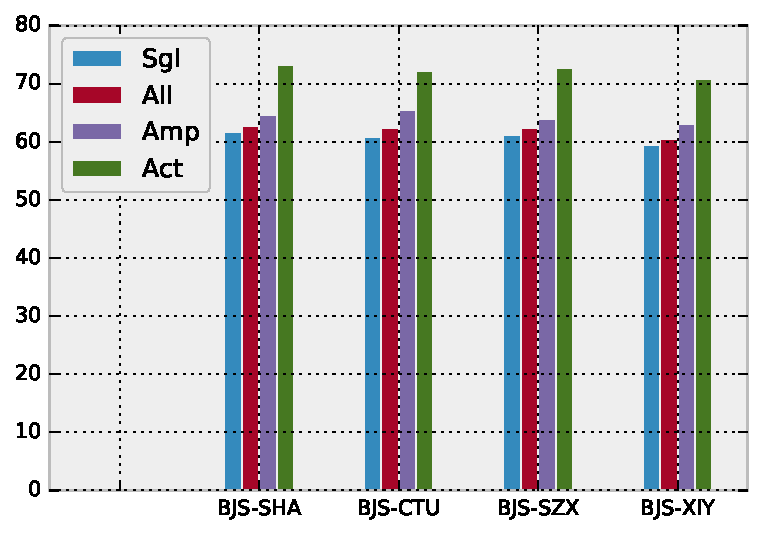
\includegraphics[width=0.75\linewidth]{06/10_res_of_cold_rec.pdf}
 \bicaption[fig:real_cold_flight]{冷启动用户推荐}{冷启动用户推荐结果}{Fig}{Mean Accuracy of Recommendation for Cold Start Users}
\end{figure}

图\ref{fig:real_cold_flight}展示了为冷启动用户在四条航线上机票推荐的结果。同样地Act标签代表为该航线活跃用户的单一航线模型推荐结果。Sgl标签为冷启动用户使用单一航线模型的推荐结果;All标签对应为冷启动用户使用全航线模型的推荐结果;Amp代表为冷启动用户基于社会关系进行模型增强的推荐结果。可以看到,为冷启动用户进行模型增强的机票推荐结果仍优于仅使用用户本身数据的单一航线用户模型和全航线用户模型。验证了具备社会关系的用户之间的偏好模型可以进行迁移,并适用于增强冷启动用户的特征分布模型,最终提高机票推荐的准确率。


\section{本章小结}
本章我们提出并分析了机票推荐场景中的冷启动问题。首先,我们基于机票的几个特征分析了航线间的分布差异及用户行为的差异。然后分析了航线差异对推荐结果的影响,当用户在目标航线上训练订单较少时,学习的特征分布模型具有一定偶然性,因而使用全航线模型的推荐效果好于单一航线模型;随着训练订单数量的增加,单一航线模型的推荐效果好于全航线模型。因此验证了对用户模型分航线的必要性。因而,可能产生几种用户冷启动问题。

第一种是用户在目标航线上的训练订单数量不足,而在别的航线上有一定数量的训练订单。这类用户称为航线冷启动用户。我们的解决策略是关注用户在其他航线上的特征分布模型,通过比较航线间的相似度,选出最优相似航线。提出了模型修正与融合的过程,得到最终的用户修正混合模型。实验结果验证了这种模型的推荐效果好于全航线模型,也进一步证明了为用户进行偏好建模时,使用的数据不一定越多越好。

第二种是用户在所有航线上的训练订单数量都不足,对于这类用户,似乎只能使用全航线模型。但是我们通过分析机票数据发现,用户与乘客并不是严格一一对应的。可以通过用户之间的共同乘客为用户建立社会关系。另外,我们还挖掘了用户间的的同乘关系。结合用户的这两种社会关系,我们提出了增强用户模型的算法,提升了这类用户的推荐效果。

对于不满足构建修正混合模型以及通过社会关系进行模型增强的用户,我们的建议是使用全航线模型进行推荐,推荐效果也会好于单一航线模型。